% 2021 新高考Ⅱ卷 19：四棱锥 Q-ABCD，底面为正方形
% 绘制依据：源 PDF 原图方位——A 后方偏左、B 左前、C 右前、D 右；QA、QD 为虚线。
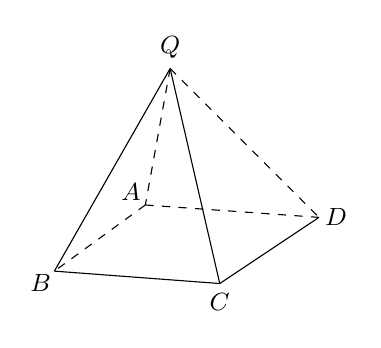
\begin{tikzpicture}[scale=1.05, font=\small]
  \coordinate (Q) at (1.75,2.6);
  \coordinate (A) at (1.45,0.95);
  \coordinate (B) at (0.35,0.15);
  \coordinate (C) at (2.35,0);
  \coordinate (D) at (3.55,0.8);
  \draw (Q) -- (B)  (Q) -- (C);
  \draw (B) -- (C) -- (D);
  \draw[dashed] (Q) -- (A)  (Q) -- (D);
  \draw[dashed] (A) -- (B)  (A) -- (D);
  \node[above] at (Q) {$Q$};
  \node[above left, inner sep=1.5pt] at (A) {$A$};
  \node[below left, inner sep=1pt] at (B) {$B$};
  \node[below] at (C) {$C$};
  \node[right, inner sep=2pt] at (D) {$D$};
\end{tikzpicture}